\section{System Design}
\label{sec:system}

This section presents the system design and implemetation of
\name.

\subsection{Centralized control of \name}
\label{subsec:system:centralized}

\begin{figure}[t]
  \centering
  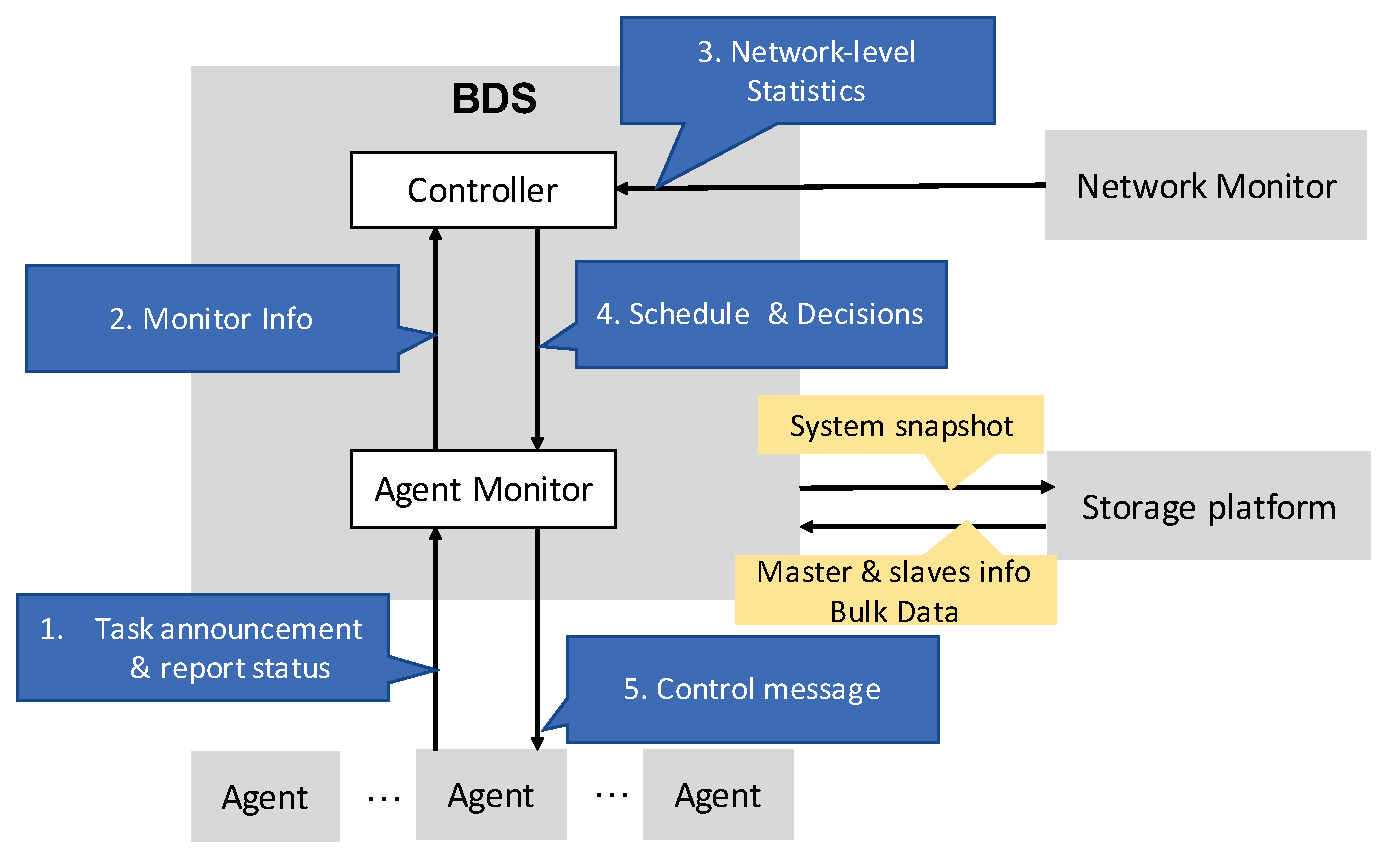
\includegraphics[width=3in]{images/implementation_v4.eps}
  \tightcaption{Interfaces of \name's centralized control.}
% \jc{please add the step of network monitor. see the new text}\jc{where are servers? avoid notions never defined before like "task announcement"}
  \label{fig:implementation}
\vspace{-0.4cm}
\end{figure}
%\vspace{-15pt}

\name periodically (by default, every three seconds) updates the
routing and scheduling decisions in a centralized fashion.
Figure \ref{fig:implementation} outlines the workflow in each
three-second cycle.
\begin{enumerate}
\item It starts with the {\em Agent}, running local on each server,
checking the local states, including data block delivery status
(which blocks have arrived, and which blocks are outstanding),
server availability, and disk failures, etc.
\item These statistics are then wrapped in a {\em control message},
and sent to the centralized {\em \name Controller} via an efficient
messaging layer called {\em Agent Monitor}.
\item The \name Controller also receives network-level statistics
(the bandwidth consumption by latency-sensitive traffic and the
utilization on each inter-DC link) from a {\em Network Monitor}.
\item On receiving the updates from all Agents and the Network
Monitor, the \name Controller runs the centralized decision-making
algorithm (\Section\ref{sec:logic}) to work out the new scheduling
and routing decisions, and sends the difference between the new
decision and the previous one to the per-server local Agent via
the Agent Monitor messaging layer.
\item Finally, the Agent allocates bandwidth for each data transfer,
and carries out the actual data transfers according the Controller's
routing and scheduling decisions.
\end{enumerate}

%It consists of four main components: {\em \name Controller},
%{\em Agent  Monitor}, {\em Agent}, and {\em Network Monitor}.
%The \name Controller runs centralized the scheduling and routing
%algorithm (\Section\ref{sec:logic}) every three seconds to update the
%routing and scheduling decisions. An Agent is a program running on
%each server to send per-server local status (such as block delivery
%status, server availability, etc), allocate bandwidth for each data
%transfer, and carry out the actual data transfers according the
%Controller's routing and scheduling decisions. The Agent Monitor is
%a messaging layer that relays the {\em control messages} between the
%Controller and Agents.
%Finally, the Network Monitor monitors the bandwidth
%consumption by latency-sensitive traffic and the utilization on each
%inter-DC link. Note that the Netowrk Monitor and Agent Monitor can be
%implemented with standard techniques (\Section\ref{sec:deployment}).
%The Network Monitor can be implemented by gathering statistics from
%routers and switches using existing APIs. \name re-uses \company's
%existing monitoring infrastructure, so we will not discuss it in
%details here.}.

%\subsection{Centralized control}
%\label{subsec:system:centralized}

%The \name Controller updates its routing and scheduling decisions
%every 3 seconds. The control interfaces between the controller and agents are two-fold: the {\em measurement collection} from agents to the controller, and the {\em control messages} from the controller to agents. The basic workflow in one cycle is following: (1) the local agent on each server checks the block status, records the IDs of blocks that finished downloading in the last cycle, and then reports the information to the agent monitor; (2) Agent Monitor aggregates the information from all the agents, updates the block delivery status and server availability status (e.g., running state, disk state, etc.), and then sends the updated information to the controller; (3) the controller runs the centralized scheduling algorithm, works out the scheduling and routing results, and sends them to the agent monitor; (4) agent monitor then forwards the control messages back to the corresponding local agents; finally, (5) the local agent sets the transmission parameters (e.g., transmission rate) according to the received control message.
%\jc{the para needs a clearer message: how centralized control is implemented? what's the data collection interface? what's the control interface? Don't use mathmatical notations (again don't assume people have read section 4) or protocols like http post (they belong to implementation).}

\name uses two additional optimizations to make the workflow
more efficient.
\begin{itemize}
\item \emph{Blocks merging}.
To reduce the computational scale and achieve more efficient
transmissions, \name merges the blocks with the same source and
destination into one subtask. Its benefits are two-fold: (1) it
significantly reduces the number of pending blocks in each
scheduling cycle, thus reducing the computational cost of the
centralized decision-making logic; and (2) it reduces the number
of parallel TCP connections between servers, which could
otherwise reduce link utilization and degraded performance.
%There are two advantages: reducing the computation scale and achieving higher-efficient transmissions. To be specific: 1) there will be a large number of pending blocks in each scheduling cycle, making calculation on the controller computationally hard to finish within an acceptable time, while block merging can significantly reduce the block number and thus reduce the calculation scale; 2) concurrent transmission will make all blocks establish connections at the same time, sharing the limited bandwidth and thus cannot possibly be finished in one cycle. This will result in connection hanging and inefficient transmissions.
\item \emph{Non-blocking update}.
To not be blocked by the controller decision-making logic, each
local Agent  keeps the ongoing data transmissions alive while the
Controller runs the centralized decision-making logic.
Consequently, Controller takes this into account by speculating the
data delivery status of each server by the time it has re-calculated
the decisions, and uses these speculated data delievery status as
the input of the centralized logic.
\end{itemize}

%\begin{itemize}
%
%\item Start with the basic workflow of each 3-second cycle: (1) how local agent collects delivery status, (2) send messages to the controller, (3) controller runs the algorithm, (4) control message to each local agent, and (5) how local agent enforce decision.
%
%\item Fault tolerance: what if a server is not available (or straggling), what if one controller instance is not available, what if there is network partition between DCs or between DCs and the controller.
%
%\item Explain two optimizations:
%\begin{itemize}
%\item Merging blocks
%\item Non-blocking update
%\end{itemize}
%
%\end{itemize}

\subsection{Dynamic bandwidth separation}
\label{subsec:system:separation}

%\jc{please mention 80\% utilization upper bound and why the conservative use of bandwidth can protect transient online flows}

To guarantee dynamic bandwidth separation between inter-DC
bulk-data multicasts and delay-sensitive traffic, \name Network
Monitor monitors the aggregated bandwidth usage of all
latency-sensitive flows on each inter-/intra-DC link, and
dynamically allocates the bandwidth of each inter-DC multicast
transfer.
%Because \name updates routing decision every few seconds,
%we reserve 20\% of link capacity to protect online flows
%from transient traffic bursts,
To protect delay-sensitive flows from bursty bulk-data transfers,
\company uses 80\% link utilization as a ``safety threshold'',
i.e., the total bandwidth consumption of bulk-data transfers
cannot exceed 80\% of the link capacity on any link.

%With the known link capacity and the aggregated size of latency-sensitive traffic, the residual bandwidth for background data can then be calculated by the difference.

%So that the reserved 20\% link capacity can absorb the traffic jitters, mask the network degradation and ensure the online-server performance. In the server end, each agent enforces the bandwidth limits by Linux Traffic Control (\texttt{tc}). Thus, \name achieves the bandwidth separation dynamically and in real-time.
%\jc{move tc stuff to implementation.}

%Such dynamic bandwidth separation scheme is different from the traditional priority-based techniques (such as \cite{kumar2015bwe}), which sets higher priority to online latency-sensitive traffic than background traffic. When traffic bursts, such priority-based techniques work as usual and allocate bandwidth according to traffic priorities, no matter whether the online traffic is suffering from high latency. As such situation can be avoided in \name, which dynamically monitors the aggregated bandwidth occupied by delay-sensitive applications and reserves enough bandwidth for them, \name guarantees the performance of latency-sensitive applications by leveraging dynamic bandwidth separation.

The dynamic bandwidth separation of \name enjoys two advantages. (1) It uses global coordination to achieve more efficient bandwidth utilization. The traditional priority-based techniques (such as \cite{kumar2015bwe}) that set higher priority to online latency-sensitive traffic than background traffic cannot react to the dynamic network environment, resulting in bandwidth wastage or performance interference. While \name can dynamically monitor the aggregated bandwidth occupied by delay-sensitive applications, and reserves moderate amounts of bandwidth for them.
(2) \name, which optimized the application-level overlay, is complementary to network-layer techniques that improve the WAN performance and fairness \cite{chen2012design, kavulya2010analysis, mishra2010towards, reiss2012heterogeneity}.
%The prior WAN optimization solutions (e.g., traffic engineering studies \cite{chen2012design, kavulya2010analysis, mishra2010towards, reiss2012heterogeneity}) have substantially improved inter-DC applications' performance, while \name's benefits of an application-level overlay network are orthogonal to these works.

%\jc{not sure the logic flows. use this flow instead: (1) bds's app-level bandwidth allocation is complementary to QoS solutions, (2) bds uses global coordination to achieve more efficient bandwidth utilization}

%\jc{please put this solution into context. what's the diff to priority-based techniques such as bwe?}


\subsection{Fault tolerance}
\label{subsec:system:fault}
Next we describe how \name handles the following failures.
%To make \name fault tolerant, the following scenarios are considered.% and the corresponding evaluations are in \Section\ref{subsubsec:evaluation:adaptability}.

\begin{packedenumerate}
\item \emph{Controller failure:} The controller is replicated using standard schemes~\cite{lamport1998part}. If the master controller fails, another replica will be elected as the new controller. If the network partition happens between DCs and the controller or when all controller copies fail, the agents running in servers will fallback to the current decentralized overlay protocol as default to ensure graceful performance degradation.
\item \emph{Server failure:} If the agent on server is still able to work, it will report the abnormal state (e.g., server crash, disk failure, etc.) to the agent monitor. Otherwise, the servers that selected this server as data source would report the unavailability to the agent monitor. In either case, the controller will remove that server from the potential data sources in the next cycle.
%\item \emph{What if there is network partition between DCs or between DCs and the controller?} If network partition happens between DCs and the controller, the whole network will fall back to a default decentralized overlay protocol to ensure graceful performance degradation. If network partition happens between DCs, the DCs located in the same partition with the controller will work the same as before, while the separated DCs will fall back to the decentralized overlay network.
\item \emph{Network partition between DCs:}
If network partition happens between DCs, the DCs located in the same partition with the controller will work the same as before, while the separated DCs will fallback to the decentralized overlay network.
\end{packedenumerate}
%
%\begin{itemize}
%
%\item First, how to get real-time aggregated size of latency-sensitive traffic.
%
%\item Second, how to calculate the bandwidth cap for background bulk traffic
%
%\item Finally, how to enforce the bandwidth cap.
%
%\end{itemize}



